\documentclass[pdf]{beamer}
\usepackage[english,vietnamese]{babel}
\usepackage{amsmath}
\usepackage{booktabs}
\usepackage{graphicx}
\usepackage{hyperref}
\usepackage{lmodern}
\usepackage{siunitx}

\mode<presentation>{}
\usetheme[hideothersubsections]{Hannover}
\usecolortheme{crane}
\usefonttheme[onlymath]{serif}
\usebackgroundtemplate{
  
\includegraphics[width=\paperwidth,height=\paperheight]{USTH.jpg}}
\renewcommand{\thefootnote}{\fnsymbol{footnote}}
\setcounter{tocdepth}{2}

\title{Satellite Internet}
\author[Group 1]{Nguyễn Như Hiếu---BI9-103\\
                 Ngô Ngọc Đức Huy---BI9-119\\
                 Ngô Xuân Minh---BI9-167\\
                 Nguyễn Gia Phong---BI9-184\\
                 Nguyễn Hồng Quang---BI9-194\\
                 Trần Minh Vương---BI9-239}
\institute{University of Science and Technology of Hà Nội}
\date{\selectlanguage{english}\today}

\begin{document}
\frame{\titlepage}
\selectlanguage{english}
\begin{frame}{Contents}
  \tableofcontents
\end{frame}

\section{Introduction}
\frame{\tableofcontents[currentsection]}
\begin{frame}{Usage}\Large
  \begin{block}{Popular Use}
    \begin{itemize}
      \item Airplane
      \item Cruise Ship
      \item Rural Area
    \end{itemize}
  \end{block}
  \begin{block}{Similarity}
    All three are either in or travel through area \\
    with little to no ground station.
  \end{block}
\end{frame}

\begin{frame}{Future Usage}\Large
  Provide Internet for the whole world

  \begin{block}{Fact}
    Over 3.7 Billion people are living without being \\
    connected to the internet.
  \end{block}
\end{frame}

\section{How It Works}
\frame{\tableofcontents[currentsection]}
\begin{frame}{Components}
  \begin{itemize}\Large
    \item Geostationary satellite (GEO)
    \item Gateway
    \item Antenna
    \item Others:
      \begin{itemize}\Large
        \item Modem
        \item Centralized NOC
      \end{itemize}
  \end{itemize}
\end{frame}

\begin{frame}{Components Interaction}
  \begin{figure}
    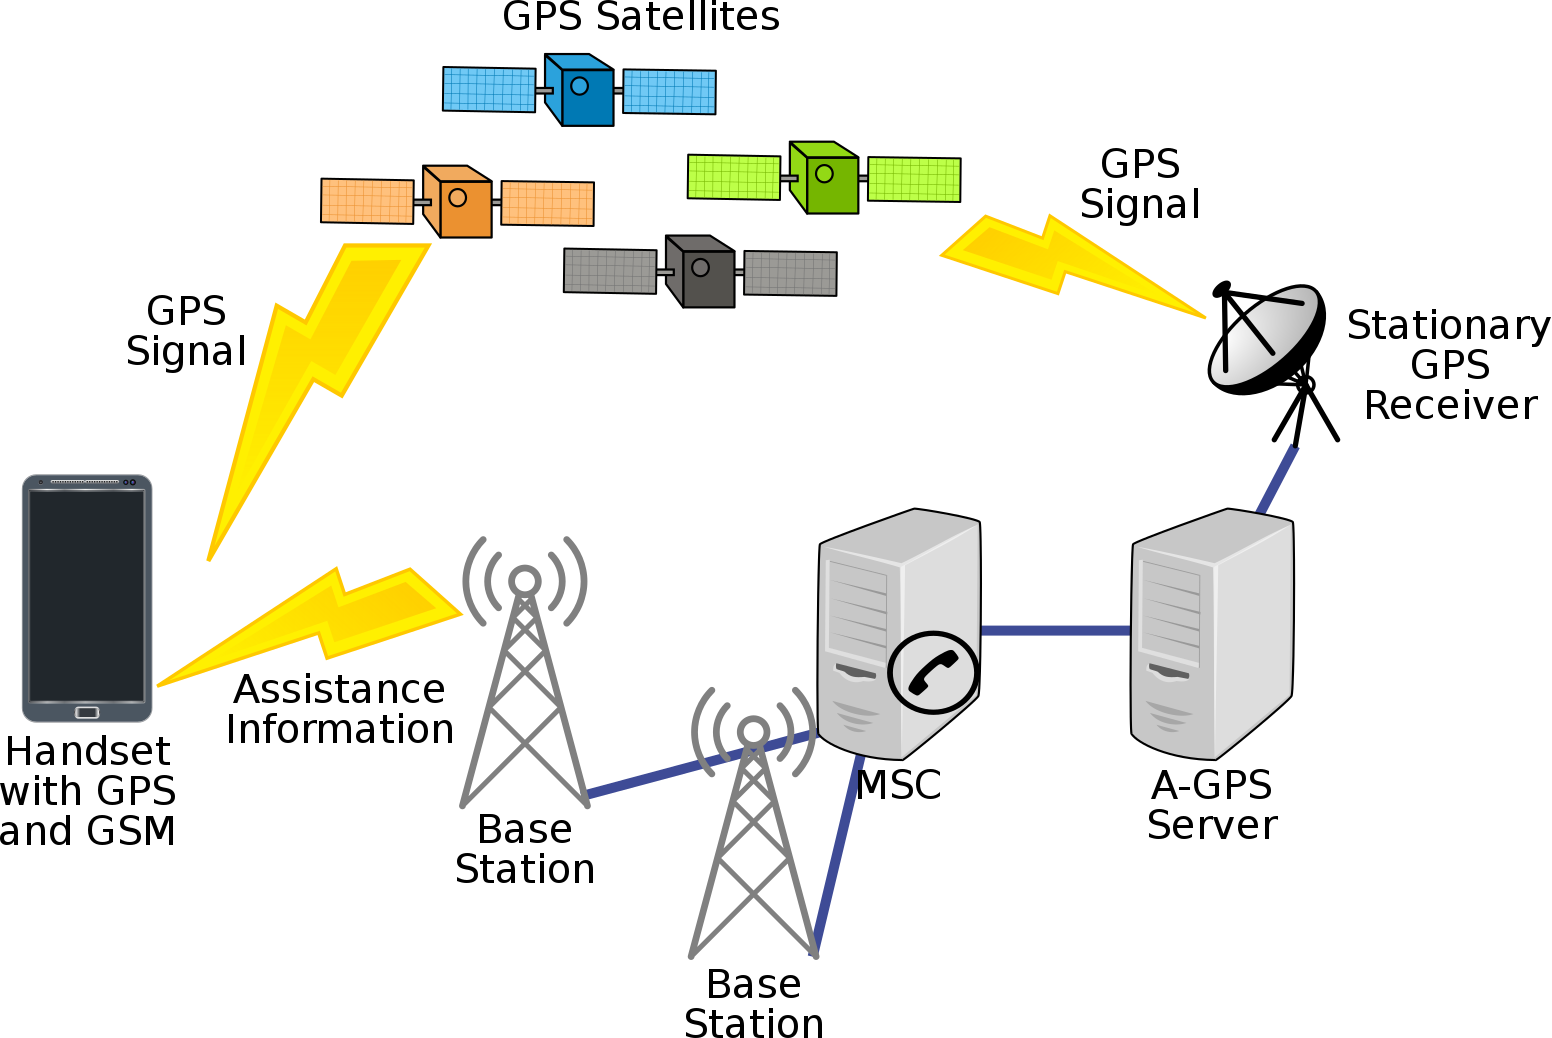
\includegraphics[width=0.9\textwidth]{A-GPS.png}
    \caption{GPS using A-GPS and GSM network}
  \end{figure}
\end{frame}


\begin{frame}{One-way Satellite Network}
\Large
  \begin{center}
    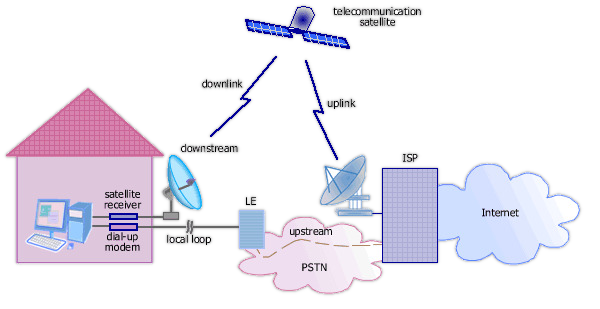
\includegraphics[width=\textwidth]{one-way-to-earth.png}
  \end{center}
\end{frame}

\subsection{1-way from Earth}
\begin{frame}{Components}\large
  \begin{itemize}
    \item Upstream: Data travelling through telephone modem
    \item Downstream: Download through satellite
  \end{itemize}
\end{frame}

\begin{frame}{Characteristics}
  \begin{itemize}
    \item Upload speed: Same as that of the dial-up internet
    \item Download speed: Much faster than dial-up internet
    \item Latency: Still high,much lower than two way satellite internet
    \item You have to tie up the telephone lie when you use the Internet
  \end{itemize}
\end{frame}

\subsection{1-way to Earth}
\begin{frame}{One-way to Earth}\Large
  \begin{block}{Components}
    \begin{itemize}
      \item 1 transmitting hub station (usually very large)
      \item Multiple receive-only Earth stations
    \end{itemize}
  \end{block}
\end{frame}

\begin{frame}{Characteristics}\Large
  \begin{itemize}
    \item Usage: IP multicast-based data,\\
      audio and video distribution
    \item Interactivity: Little user interface,\\
      similar to TV or radio content
  \end{itemize}
\end{frame}

\subsection{2-way}
\begin{frame}{Two-way Satellite Network}
  \begin{center}
    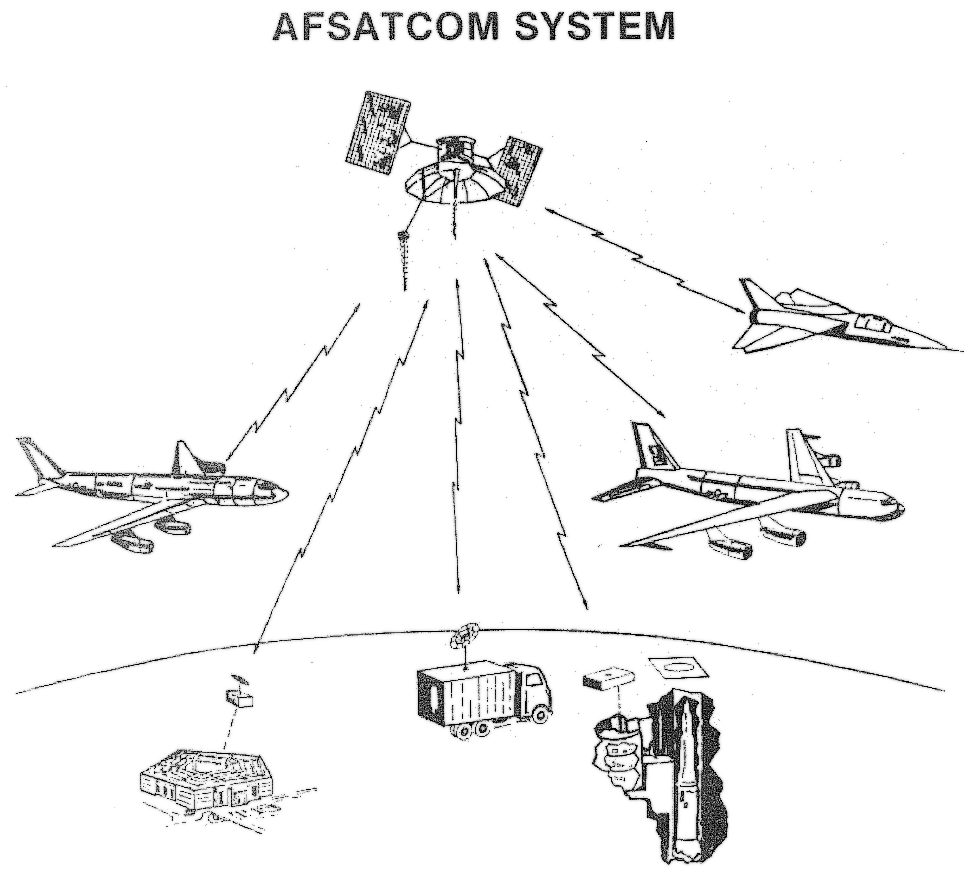
\includegraphics[width=0.8\textwidth]{two-way.png}
  \end{center}
\end{frame}

\begin{frame}{Components}\LARGE
  \begin{itemize}
    \item VSAT: Send and receive data
    \item Telecommunication port:\\ Relay data through Internet
  \end{itemize}
\end{frame}

\begin{frame}{Condition}\LARGE
  Satellite dish must be precisely pointed\\
  to avoid interference.
\end{frame}

\begin{frame}{Characteristics}\large
  \begin{itemize}
    \item Both TDMA and single channel per carrier
    \item Mostly Ku-band, but also C-band and Ka-band
    \item May utilize telephone modem to reduce latency
    \item Home-user's bandwidth based on payment
    \item Difficult on moving vehicles
  \end{itemize}
\end{frame}

\begin{frame}{Portable Satellite Internet}
  \begin{block}{Portable}
    \begin{itemize}
      \item Use self-contained box pointed in general direction of Satellite
      \item Expensive
    \end{itemize}
  \end{block}
  \begin{block}{Satellite phone}
    \begin{itemize}
      \item Omnidirectional antenna so no alignment needed
      \item Low bandwidth so slow to browse net,useful for sending email
    \end{itemize}
  \end{block}
\end{frame}

\section{Limits and Challenges}
\frame{\tableofcontents[currentsection]}

\subsection{Weather}
\begin{frame}{Heavy rain or Blizzard}\LARGE
  \begin{itemize}
    \item Fading
    \item Accumulating raindrop or snow
    \item Wind
  \end{itemize}
\end{frame}

\subsection{Latency}
\begin{frame}{Latency}\large
  \begin{block}{Satellite altitude}
    \begin{itemize}
      \item LEO: $<$ \SI{2000}{\kilo\meter}
      \item MEO: 2000--\SI{35786}{\kilo\meter}
      \item GEO: $>$ \SI{35786}{\kilo\meter}
    \end{itemize}
  \end{block}
  \begin{block}{Result}
    GEO has 12 times higher latency than terrestrial base networks.
    LEO and MEO have a bit lower delay.
  \end{block}
\end{frame}

\subsection{Others}
\begin{frame}{Other Limitations}\Large
  \begin{block}{Economically}
    Costly: \SI{2}{\mega b\per\second} costs around \$100 a month.
  \end{block}
  \begin{block}{Environmentally}
    Space junk: Only 2000 out of 5000 launched satellites are still in function.
  \end{block}
\end{frame}

\section{Mitigations}
\frame{\tableofcontents[currentsection]}
\subsection{Techniques}
\begin{frame}{Fade Mitigation Techniques}\Large
  Common functions:
  \begin{itemize}
    \item \emph{Monitor} link quality by continuous measurements
    \item \emph{Predict} short-term behavior and duration\\
      of satellite channel's next state
    \item \emph{Set} parameters based on previous estimation
  \end{itemize}
\end{frame}

\subsubsection{EIRP Control Techniques}
\begin{frame}{Effective Isotropic Radiated Power}\Large
  \begin{itemize}
    \item EIRP = tranmitted power $\times$ antenna gain
    \item EIRP control = adjusting carrier power
      or antenna gain to compensate for power losses
  \end{itemize}
\end{frame}

\begin{frame}{Power Control System}
  \begin{enumerate}\large
    \item Open loop: Based on recently received power.
      \begin{itemize}\large
        \item Non-reliable
        \item Responsive
      \end{itemize}
    \item Closed loop: Based on channel power measurements.
      \begin{itemize}\large
        \item More comprehensive
        \item Large propagation delay
      \end{itemize}
  \end{enumerate}
\end{frame}

\begin{frame}{Uplink Power Control}
  \begin{itemize}
    \item Vary carrier power at the earth station
    \item Restoration of side lobes might lead to\\
      adjacent \emph{channel} interference\\
      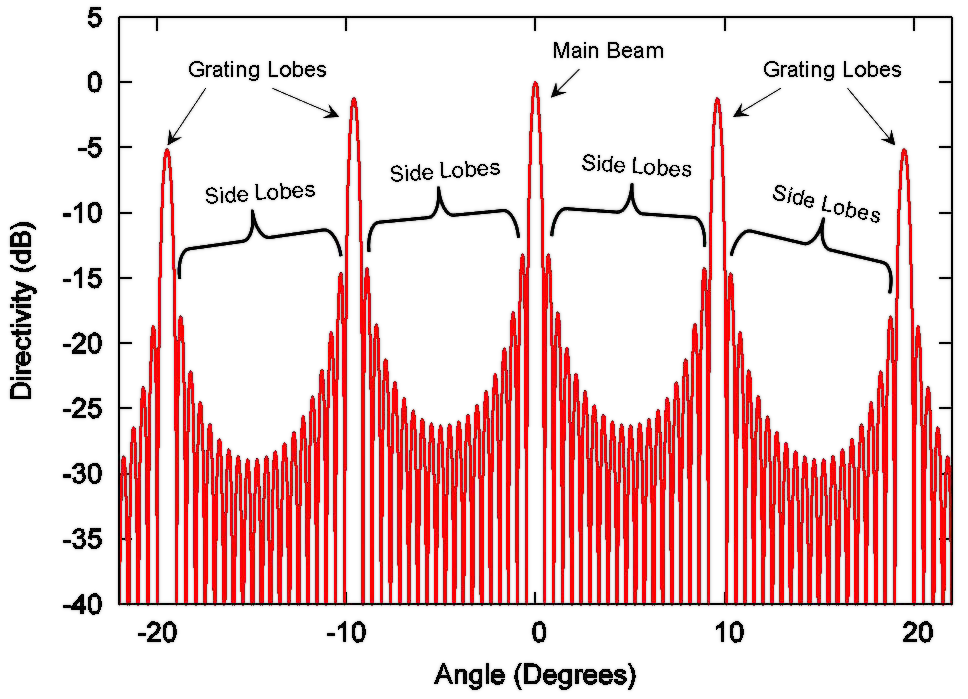
\includegraphics[width=0.54\textwidth]{lobes.png}
    \item Increase of earth station transmit power may cause
      adjacent \emph{satellite} interference\footnote{Satellites
      are separated by 2--3 degrees on the geostationary orbit.\\}
    \item Effective and preferred by many satellite operators
  \end{itemize}
\end{frame}

\begin{frame}{Downlink Power Control}
  \begin{itemize}\Large
    \item Vary carrier power on-board the satellite
    \item Difficult to implement due to\\ satellite size and weight limitations
    \item Subject to
      \begin{enumerate}\large
        \item Adjacent \emph{channel} interference
        \item Inter\emph{modulation} interference
        \item Inter\emph{system} interference (with terrestrial networks)
      \end{enumerate}
  \end{itemize}
\end{frame}

\begin{frame}{Spot Beam Shaping}\Large
  \begin{itemize}
    \item Adjust antenna gain on-board the satellite\\
      for a certain geographical region
    \item Shape satellite antenna for nearly constant\\
      ground receive power, even under rainfall
    \item Does \textbf{not} need expensive calculations\\
      for attenuation estimation\footnote{SBS compensates
      the entire coverage area instead of a single site.\\}
    \item Technology and research are WIP
  \end{itemize}
\end{frame}

\subsubsection{Adaptive Transmission Techniques}
\begin{frame}{Adaptive Transmission Techniques}
  \begin{itemize}\Large
    \item Modify processing/transmission\\ manner of signals
    \item Resource-shared techniques
    \item Categories:
      \begin{enumerate}\large
        \item Hierarchical coding
        \item Hierarchical modulation
        \item Data rate reduction
      \end{enumerate}
  \end{itemize}
\end{frame}

\begin{frame}{Hierarchical Coding}\large
  \begin{itemize}
    \item Add redundancy to the information signal
    \item Trade-off between bandwidth and error probability
    \item Different conditions require different coding schemes
    \item Prioritize users with less efficient coding schemes, i.e.\\
      longer bursts (TDMA) or larger bandwidth (FDMA)
  \end{itemize}
\end{frame}

\begin{frame}{Hierarchical Modulation}\large
  \begin{itemize}
    \item Provide lower quality fallback in case of weak signals
    \item Exchange bandwidth efficiency for power requirements
    \item Suitable for localized satellite systems, e.g. VSAT
    \item Users with lower-order modulation get more resources
  \end{itemize}
\end{frame}

\begin{frame}{Data Rate Reduction}\large
  \begin{itemize}
    \item Reduce information data rate for power gain
    \item Distribute satellite resources equally to every user
    \item Utilizable where significant information rate reduction\\
      is tolerable, e.g.\ video or data but voice transmission
  \end{itemize}
\end{frame}

\subsubsection{Diversity Protection Schemes}
\begin{frame}{Diversity Protection Schemes}\large
  \begin{itemize}
    \item Use multiple channels with different characteristics
    \item Oriented against rain fades and highly efficient
    \item Performance criteria
      \begin{itemize}
        \item Diversity gain: difference between site attenuation\\
          and joint attenuation, for the same probability level
        \item Diversity improvement: ratio of site exceedence probability
          to the joint one, for the same attenuation value
      \end{itemize}
  \end{itemize}
\end{frame}

\begin{frame}{Diversity Techniques}
  \begin{tabular}{l p{0.39\textwidth} l p{0.18\textwidth}}
    \toprule
    \textbf{Diversity} & \textbf{Setup} & \textbf{Efficiency} & \textbf{Cost}\\
    \midrule
    Site & Connected earth stations & High & High\\
    Orbital & Earth station may choose\newline between satellites & Low & Low\\
    Frequency & Use lower frequency\newline on higher attenuation
              & Adaptive & Terrestrial equipments\\
    Time & Repeat faded data & Selective\footnote{\ldots of fade duration} & N/A\\
    \bottomrule
  \end{tabular}
\end{frame}

\subsection{Comparison}
\begin{frame}{EIRP Control Techniques}
  \begin{table}
    \begin{tabular}{l l p{0.27\textwidth} p{0.2\textwidth}}
      \toprule
      \textbf{Tech} & \textbf{Availability}
      & \textbf{Max gain} (dB) & \textbf{Cons} \\
      \midrule
      ULPC & 0.01--10 \% & 5 (VSAT)\newline 15 (hubs)& power range \\
      DLPC & 0.01--10 \% & 3 (sat.~TWTA) & power range \\
      SBS & 0.01--1 \% & 5 (sat.~antenna) & immature research \\
      \bottomrule
    \end{tabular}
    \caption{Comparisons between EIRP control techniques}
  \end{table}
\end{frame}

\begin{frame}{Adaptive Transmission Techniques}
  \begin{table}
    \begin{tabular}{l l p{0.25\textwidth} p{0.23\textwidth}}
      \toprule
      \textbf{Tech} & \textbf{Availability}
      & \textbf{Max gain} (dB) & \textbf{Cons} \\
      \midrule
      HC/HM & 0.01--10 \% & 10--15\newline ($E_b/N_0$ range)
      & fading in \newline many stations \\
      DDR & 0.01--10 \% & 3--9 & low rate\newline intolerant \\
      \bottomrule
    \end{tabular}
    \caption{Comparisons between adaptive transmission techniques}
  \end{table}
\end{frame}

\begin{frame}{Diversity Protection Schemes}
  \begin{table}
    \begin{tabular}{l l p{0.25\textwidth} p{0.24\textwidth}}
      \toprule
      \textbf{Tech} & \textbf{Availability}
      & \textbf{Max gain} (dB) & \textbf{Cons} \\
      \midrule
      SD & 0.001--0.1 \% & 10--30\newline (conv.~rain) & cost \\
      OD & 0.001--1 \%  & 3--10 & satellite switch \\
      FD & 0.01--10 \% & 30 (Ka--Ku) & cost\\
      \bottomrule
    \end{tabular}
    \caption{Comparisons between diversity protection schemes}
  \end{table}
\end{frame}

\section{Conclusion}
\frame{\tableofcontents[currentsection]}
\begin{frame}{Conclusion}\LARGE
  \begin{itemize}
    \item Have many potentials
    \item Challenging
    \item Need more research
  \end{itemize}
\end{frame}

\begin{frame}{References}
  \begin{thebibliography}{69}
    \setbeamertemplate{bibliography item}[article]
    \bibitem{KuKaV} Athanasios D.~Panagopoulos,\\
      Pantelis-Daniel M.~Arapoglou and Panayotis G.~Cottis.\\
      ``Satellite communications at Ku, Ka, and V bands:
      Propagation impairments and mitigation techniques''.\\
      \emph{Communications Surveys \& Tutorials}, vol.~6, p.~2--14.\\
      IEEE, 2004.  doi:10.1109/COMST.2004.5342290. 
    \setbeamertemplate{bibliography item}[online]
    \bibitem{wiki} Satellite Internet access.  \emph{Wikipedia}.
  \end{thebibliography}
\end{frame}

\begin{frame}{Copying}\Large
  \begin{center}
    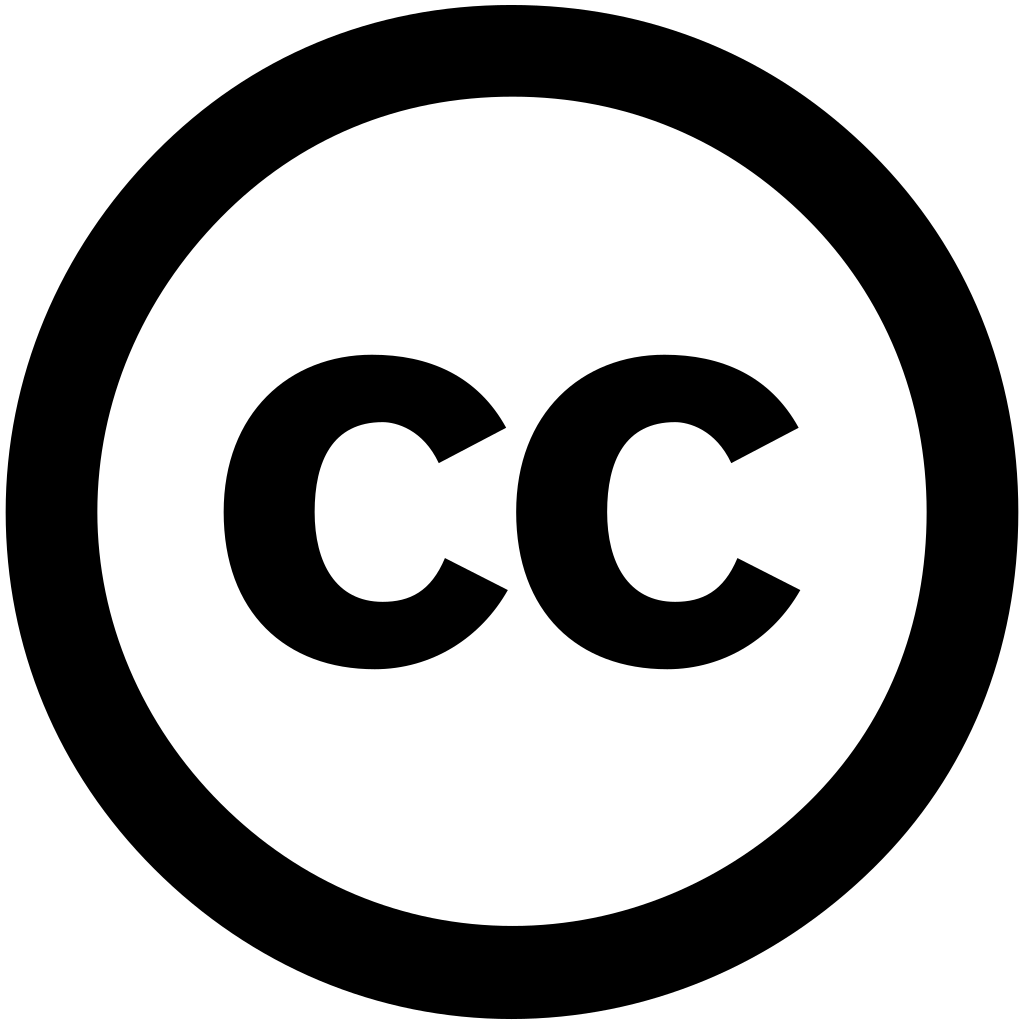
\includegraphics[width=0.2\textwidth]{CC.png}
    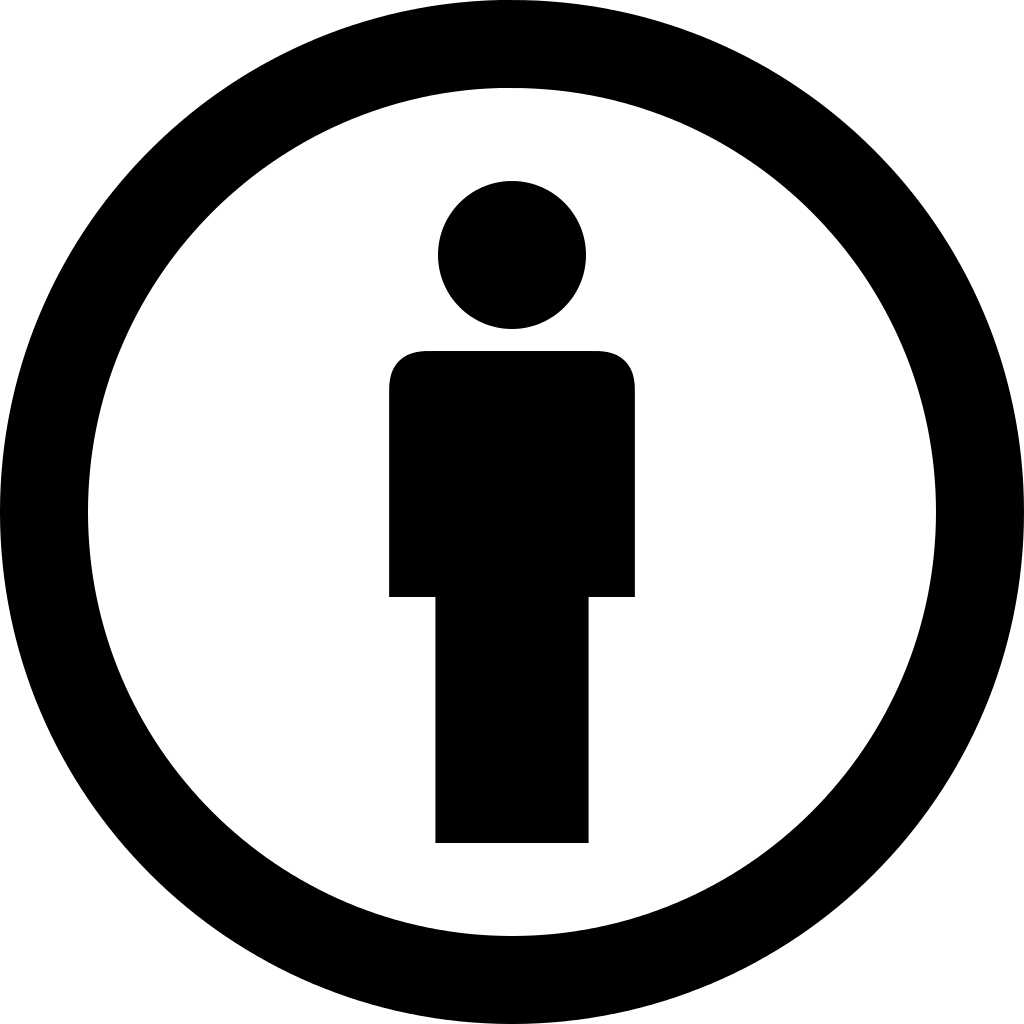
\includegraphics[width=0.2\textwidth]{BY.png}
    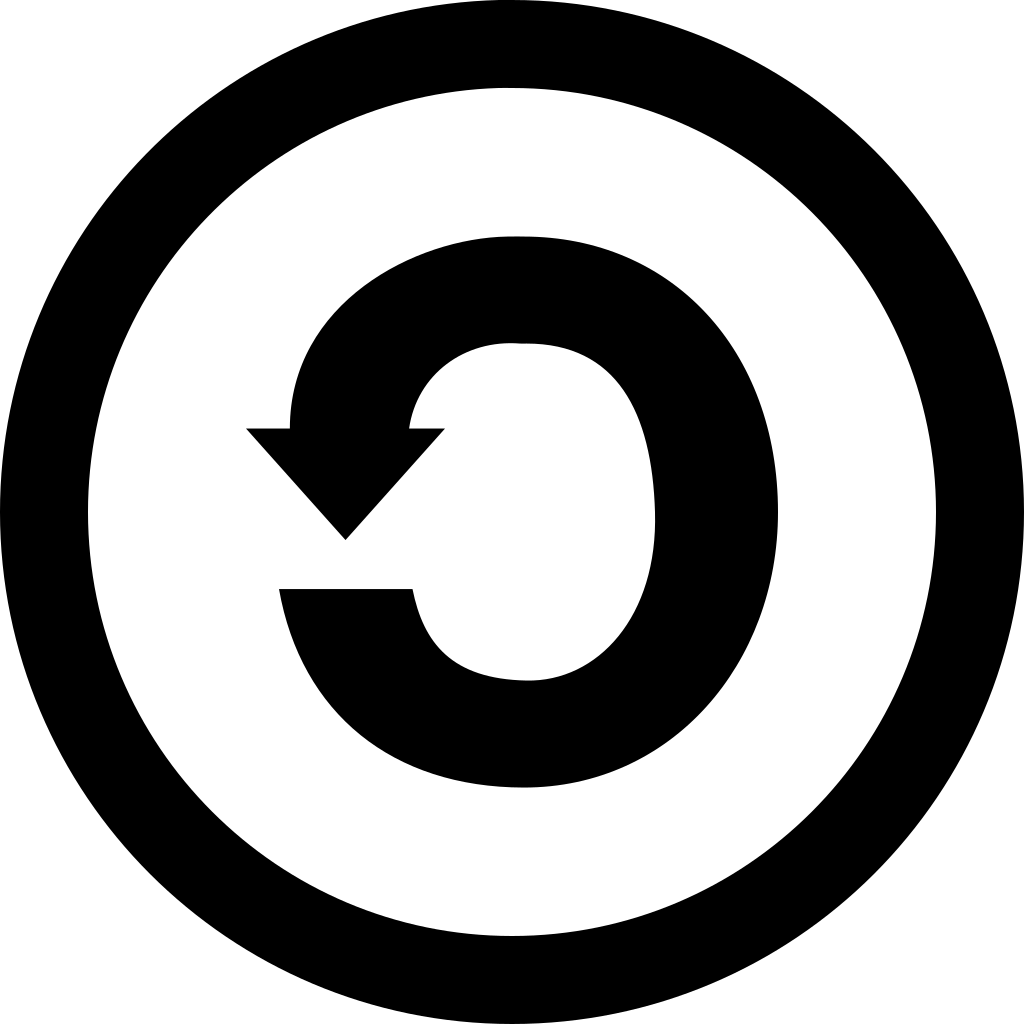
\includegraphics[width=0.2\textwidth]{SA.png}
  \end{center}

  This work is licensed under a
  \href{https://creativecommons.org/licenses/by-sa/4.0/}{Creative Commons
  Attribution-ShareAlike 4.0 International License}.
\end{frame}
\end{document}
